\documentclass[conference]{IEEEtran}
\IEEEoverridecommandlockouts

\usepackage{cite}
\usepackage{amsmath,amssymb,amsfonts}
\usepackage{algorithmic}
\usepackage{algorithm}
\usepackage{graphicx}
\usepackage{textcomp}
\usepackage{xcolor}
\usepackage{booktabs}
\usepackage{url}
\usepackage{pgfplots}
\usepackage{tikz}
\usepackage{pgfplotstable}
\pgfplotsset{compat=1.18}
\usetikzlibrary{positioning}
\graphicspath{{../figures/}{figures/}}

\def\BibTeX{{\rm B\kern-.05em{\sc i\kern-.025em b}\kern-.08em
    T\kern-.1667em\lower.7ex\hbox{E}\kern-.125emX}}

% Shared math shortcuts used across sections.
\newcommand{\nvec}{\hat{\mathbf{n}}}
\newcommand{\zhat}{\hat{\mathbf{z}}}
\newcommand{\R}{\mathbb{R}}

\begin{document}

\title{Comparative Evaluation of Classical Geometric Methods for
Steppable-Surface Segmentation in Simulated Staircase Point Clouds}

\author{\IEEEauthorblockN{Riyadh Lakadimu}
\IEEEauthorblockA{\textit{Master Program in Electrical Engineering} \\
\textit{Politeknik Elektronika Negeri Surabaya (PENS)}\\
Surabaya, Indonesia \\
riyadhlakadimu724@gmail.com}}

\maketitle

\begin{abstract}
Reliable identification of steppable surfaces is a prerequisite for
stair-climbing and stair-following robots. This paper presents a controlled,
fully labeled benchmark for steppable-surface segmentation built from a
parametric mathematical model of a four-step staircase point cloud with
LiDAR-style noise and outliers, and a systematic comparison of four classical
geometric segmentation methods: orientation-gated RANSAC plane fitting,
PCA-based normal analysis, orientation-aware DBSCAN clustering with slope
analysis, and height-histogram analysis. On a cloud of 18{,}333 points, the
DBSCAN-with-slope method attained the highest tread-class scores
(F1~$=0.943$, IoU~$=0.892$), followed closely by PCA normal analysis
(F1~$=0.927$). Plain RANSAC was the least precise because horizontal plane
hypotheses absorb riser points at tread heights. A noise-sensitivity study
shows the tread-class F1 degrading from $0.956$ to $0.543$ as the height
noise $\sigma_z$ grows from $0.01$\,m to $0.07$\,m. We discuss the safety
implications of these error modes for robotic stair traversal and argue for
ensemble fusion with safety margins. The benchmark, code, and equations are
released to support reproducible comparison.
\end{abstract}

\begin{IEEEkeywords}
point cloud, segmentation, RANSAC, PCA, DBSCAN, staircase, mobile robot,
traversability, LiDAR
\end{IEEEkeywords}

\section{Introduction}
Robots that climb or follow staircases, along with assistive devices for
the visually impaired, must reason about three-dimensional structure to
act safely. Legged and wheeled platforms increasingly depend on
egocentric depth sensing to negotiate stairs and other discontinuous
terrain \cite{agarwal2022legged,belter2016adaptive,stelzer2012stereo}.
Shared-autonomy systems likewise demand reliable geometric cues before a
foot or wheel is committed to a surface \cite{marion2017director}. Across
all of these settings the central perceptual question stays the same:
which parts of an observed point cloud form a \emph{tread}, the steppable
horizontal surface on which weight can be safely placed, and which form a
near-vertical \emph{riser} or are simply spurious edge and outlier
returns.

The problem is safety-critical. Labeling a tread as non-steppable only
sacrifices an option, but labeling a riser or edge as steppable invites a
foothold onto a vertical face, which produces slips, stumbles, or falls.
The same hazard motivates stair perception for the visually impaired,
where undetected steps are a recognised fall hazard behind dedicated
stair-detection systems \cite{matsumura2022deep}. Reliable tread
detection therefore needs high recall and, just as importantly, high
precision on the steppable class.

Recent work attacks stair and terrain perception with deep neural
networks that learn point-wise semantics directly from raw clouds
\cite{qi2016pointnet,matsumura2022deep}. These methods are powerful but
data hungry. They require large volumes of densely labeled
three-dimensional scans, which are costly to acquire for the specific
geometry of stairs, and they offer limited interpretability. The tread
sub-problem also lacks controlled, reproducible benchmarks with exact
ground-truth labels, so reported results are hard to compare across
studies. Classical geometric methods are fast, transparent, and
label-free by contrast. Yet despite their maturity in plane segmentation
and traversability estimation
\cite{chavezgarcia2017learning,gomes2023survey}, they remain
under-compared on the staircase setting under matched conditions.

We address this gap with a controlled, fully reproducible study of
classical geometric segmentation for steppable-surface detection on
staircases. Our contributions are as follows:
\begin{itemize}
  \item A parametric, fully labeled staircase point-cloud generator that
        emits exact tread, riser, and other labels while modeling LiDAR
        range jitter and outliers, enabling reproducible evaluation.
  \item A unified three-class problem formulation together with the
        implementation of four classical methods under a common
        orientation-aware pipeline: RANSAC plane fitting, PCA normal
        analysis, DBSCAN with slope confirmation, and a height-histogram
        level detector.
  \item A quantitative comparison of all four methods on the steppable
        (tread) class, accompanied by a controlled noise-sensitivity
        study that characterizes degradation as height noise grows.
  \item A safety-oriented discussion of the results for robotic stair
        traversal, relating precision and intersection-over-union to the
        risk of unsafe footholds.
\end{itemize}

The remainder of this paper is organized as follows: Section~II reviews
related work, Section~III presents the proposed data generator and the
four segmentation methods, Section~IV reports the comparative evaluation
and noise study, and Section~V concludes.

\section{Related Work}
\label{sec:related}

Detecting steppable surfaces in staircase point clouds touches several
threads of point-cloud processing. We organise the literature thematically
and weigh each line of work against the requirements of our problem:
fast, interpretable, and label-free segmentation of treads and risers.

\subsection{Geometric plane segmentation}
The dominant paradigm for extracting planar structure from unorganised
clouds is Random Sample Consensus (RANSAC). Li \emph{et al.}\
\cite{li2017improved} improve standard RANSAC for indoor and urban plane
segmentation by guiding sampling with Normal Distribution Transformation
cells, which mitigates the spurious planes that plain RANSAC fits across
disjoint surfaces. The same plane-fitting machinery appears in RGB-D
object recognition \cite{jalal2021rgb} and inside real-time planar LiDAR
SLAM \cite{zhou2021lsam}, where planes act as map primitives. Such
methods are efficient and interpretable. The difficulty is that they
treat planes as generic primitives with no orientation prior. On a
staircase the globally dominant plane is the oblique ramp spanning all
steps, so unconstrained fitting absorbs riser points into tread planes.
This observation motivates the orientation gate in our pipeline.

\subsection{Normal estimation and surface analysis}
A complementary route reasons about local surface geometry rather than
global primitives. Huang \emph{et al.}\ \cite{huang2009consolidation}
consolidate unorganised clouds and estimate reliable normals for surface
reconstruction, whereas Castillo \emph{et al.}\ \cite{castillo2013point}
recover normals through constrained nonlinear least squares for joint
segmentation and denoising. Per-point normals are attractive for stairs
because tread and riser differ sharply in orientation. On its own,
though, normal estimation produces no grouping into coherent surfaces and
remains sensitive to neighbourhood scale under noise. Our PCA-normal
baseline builds directly on this principle, classifying points by the
tilt of the smallest-eigenvector normal relative to the vertical axis.

\subsection{Clustering and region growing}
To recover surfaces rather than isolated points, clustering and
region-growing methods aggregate neighbours by geometric similarity.
Density-based clustering (DBSCAN) has been used to identify and localise
3D weld seams robustly in the presence of outliers
\cite{zhou2024identification}. Euclidean clustering supports object
detection from fused sparse clouds and imagery \cite{xu2021object}, and
supervoxel-based region growing yields compact, boundary-respecting
segments \cite{luo2021supervoxel}. Approaches of this kind naturally
reject outliers as noise and form one cluster per physical surface, which
suits the discrete tread and riser structure of stairs. What they do not
encode is the horizontal-versus-vertical distinction we require, so we
precede spatial clustering with an orientation split and confirm each
cluster by its slope.

\subsection{Ground and LiDAR segmentation}
Separating traversable ground from obstacles is a long-studied special
case of surface segmentation. The survey by Gomes \emph{et al.}\
\cite{gomes2023survey} catalogues ground-segmentation methods for
automotive LiDAR and highlights a recurring trade-off: geometric methods
are fast and transparent, while learned methods are accurate but opaque.
Stairs are a structured instance of this ground-versus-non-ground
problem, in which each tread is a small, elevated ground patch rather
than a single dominant plane.

\subsection{Learning-based segmentation}
Deep networks have reshaped point-cloud semantic segmentation since
PointNet \cite{qi2016pointnet} demonstrated direct learning on raw point
sets, and recent surveys document the breadth of this progress
\cite{sarker2024comprehensive}. Because dense labels are costly, weakly
supervised \cite{li2022hybridcr}, few-shot \cite{zhao2020few}, and
prototype-based few/zero-shot \cite{he2023prototype} formulations all aim
to reduce annotation demand. Accuracy is strong, but these models stay
data-hungry, depend on representative training distributions, and offer
limited interpretability and reproducibility for a safety-critical
sub-problem such as foothold detection. That cost in data and
transparency is precisely what motivates revisiting classical geometry
for stairs.

\subsection{Robotic stair and terrain perception}
In robotics, stair and terrain perception is tightly coupled to control.
Matsumura \emph{et al.}\ \cite{matsumura2022deep} detect stairs from 3D
point clouds with deep learning to prevent falls, and operator-assisted
stair traversal has been demonstrated in field systems
\cite{marion2017director}. Legged platforms lean on elevation maps and
adaptive planning \cite{belter2016adaptive}, egocentric vision
\cite{agarwal2022legged}, and stereo-based navigation over rough terrain
\cite{stelzer2012stereo}, while traversability itself can be learned from
simulation \cite{chavezgarcia2017learning}. Such systems confirm that
reliable steppable-surface detection is a prerequisite for safe motion.
They are typically evaluated end-to-end on bespoke platforms, however,
which leaves the underlying segmentation step without an isolated,
comparable benchmark.

\subsection{Gap addressed by this work}
Across these threads, geometric methods are fast and interpretable yet
rarely compared head-to-head on stairs, while learned methods require
labelled data that is unavailable for this specific task. No prior study
offers a controlled, fully labelled staircase benchmark on which
classical segmenters can be measured against a common ground truth. We
fill this gap with a parametric, fully annotated point-cloud generator
and an apples-to-apples comparison of four classical methods for
steppable-surface detection.

\section{Proposed Method}
\label{sec:method}

This section formalises the steppable-surface segmentation problem. It then
describes a parametric generator that produces a fully labelled staircase point
cloud with realistic sensor artefacts. Finally, it details four classical
geometric methods that we implement and compare under an identical 3-class
formulation.

\subsection{Problem Formulation and Class Scheme}
We treat staircase perception as a point-wise classification problem. Given an
unorganised cloud $\mathcal{P}=\{\mathbf{x}_i\}_{i=1}^{M}$ with
$\mathbf{x}_i\in\R^3$, the goal is to assign every point a label
$\ell_i\in\{0,1,2\}$, where label $0$ denotes a \emph{tread} (a steppable,
nominally horizontal surface), label $1$ denotes a \emph{riser} (the vertical
face connecting consecutive treads), and label $2$ denotes \emph{other}
(structural edges, sensor noise, and outliers). The tread class is the primary
class of interest, since a robot or assistive device plans footholds on tread
surfaces. We therefore evaluate it in a one-vs-rest setting while still reporting
overall 3-class accuracy.

The decisive geometric cue separating the first two classes is surface
orientation relative to the vertical axis. Let $\nvec$ be the unit surface
normal at a point and $\zhat$ the world vertical. A tread satisfies
$|\nvec^\top\zhat|\to 1$ (its normal is nearly parallel to $\zhat$), whereas a
riser satisfies $|\nvec^\top\zhat|\to 0$ (its normal is nearly orthogonal to
$\zhat$). Every method below exploits this orientation contrast, either
explicitly through a normal-based gate or implicitly through the height
structure of the cloud. Treating orientation as the organising principle yields
the unified pipeline summarised in Algorithm~\ref{alg:pipeline}. Each of the four
methods plugs into this pipeline at the clustering or plane-fitting stage.

\begin{algorithm}[t]
\caption{Orientation-aware segmentation (generic)}\label{alg:pipeline}
\begin{algorithmic}[1]
\STATE estimate per-point normals $\nvec_p$ via PCA over $k$ neighbours \eqref{eq:cov}
\STATE split points into horizontal / vertical orientation groups
\STATE cluster or fit planes within each group
\STATE confirm each region by its plane tilt $|\nvec^\top\zhat|$
\STATE label tread / riser / other
\end{algorithmic}
\end{algorithm}

\subsection{Parametric Data Generation}
To obtain a controlled and fully labelled benchmark, we synthesise the staircase
analytically from physical parameters: width $w=2.5$\,m, tread depth
$d=0.30$\,m, step height $h=0.18$\,m, and $N=4$ steps. For step index
$i\in\{0,\dots,N-1\}$, tread points are sampled uniformly over the horizontal
extent of step $i$ and placed at height $ih$ with additive Gaussian height
noise following \eqref{eq:tread}:

\begin{equation}\label{eq:tread}
\begin{cases}
x \sim \mathcal{U}(0,\,w) \\
y \sim \mathcal{U}(i d,\,(i{+}1) d) \\
z = i h + \epsilon_z,\quad \epsilon_z \sim \mathcal{N}(0,\sigma_z^2)
\end{cases}
\end{equation}
\begin{equation}\label{eq:riser}
\begin{cases}
x \sim \mathcal{U}(0,\,w) \\
y = i d + \epsilon_y,\quad \epsilon_y \sim \mathcal{N}(0,\sigma_y^2) \\
z \sim \mathcal{U}((i{-}1) h,\, i h)
\end{cases}
\end{equation}

Riser points come from \eqref{eq:riser} for $i\in\{1,\dots,N-1\}$, the vertical
face rising to tread $i$. They share the same lateral spread but lie on a
vertical plane at depth $id$ with small along-depth jitter $\sigma_y=0.02$\,m,
and their height sweeps uniformly across one step rise. The nominal height noise
is $\sigma_z=0.02$\,m, which we later vary to probe sensitivity. On top of this
structured cloud we inject realism in two ways. About $4\%$ of the points are
replaced by uniformly distributed outliers spanning the staircase bounding
volume, mimicking spurious returns and edge artefacts; these carry the
\emph{other} label. Every retained point then receives an isotropic LiDAR-like
jitter drawn from $\mathcal{N}(0,0.005^2)$ on each coordinate, approximating the
few-millimetre range noise typical of indoor depth sensors. We treat this value
as a nominal modelling choice, not a calibrated sensor model, and probe its
principal axis ($\sigma_z$) directly in Section~\ref{sec:evaluation}. The
resulting cloud contains $18{,}333$ points, partitioned as $12{,}800$ tread,
$4{,}800$ riser, and $733$ other. The generator emits per-point labels by
construction, so it provides exact ground truth for both training-free
evaluation and the noise sweep. This removes the manual-annotation bottleneck
that hampers learned segmenters.

\subsection{RANSAC Plane Fitting}
The first method fits planes by Random Sample Consensus. A candidate plane with
unit normal $\nvec$ and offset $b$ scores points by their orthogonal distance.
The inlier set $\mathcal{I}$ then collects every point closer than a tolerance
$\tau$:

\begin{equation}\label{eq:plane}
d(\mathbf{x}) = |\,\nvec^\top \mathbf{x} + b\,|,\qquad
\mathcal{I} = \{\mathbf{x} : d(\mathbf{x}) < \tau\}
\end{equation}

A naive single fit fails on stairs. The dominant plane that maximises inliers is
the oblique surface spanning the entire staircase, whose normal has
$|\nvec^\top\zhat| = d/\sqrt{d^2+h^2}\approx 0.86$. RANSAC therefore returns a
spurious ``ramp'' that absorbs both treads and risers into one steppable region.
We avoid this with a two-phase, orientation-gated scheme. The first phase
extracts horizontal planes (treads) by accepting only fits whose normal
satisfies $|\nvec^\top\zhat|\ge 0.93$. The second re-runs RANSAC on the residual
points to extract vertical planes (risers) with $|\nvec^\top\zhat|\le 0.25$. We
set $\tau=0.035$\,m and impose minimum inlier counts of $2{,}000$ points for
tread planes and $300$ for riser planes. This suppresses thin riser slices from
contaminating tread fits, at the cost of occasionally rejecting sparse vertical
faces. The orientation-aware variant follows the spirit of structure-guided
RANSAC refinements~\cite{li2017improved,jalal2021rgb}.

\subsection{PCA Normal Analysis}
The second method classifies each point purely from its local surface
orientation. For point $p$ we gather its $k$ nearest neighbours
$\mathcal{N}_k(p)$ and form the local covariance matrix $\mathbf{C}_p$. The
eigenvector tied to its smallest eigenvalue serves as the surface normal:

\begin{equation}\label{eq:cov}
\mathbf{C}_p = \frac{1}{k}\sum_{j\in\mathcal{N}_k(p)}
(\mathbf{x}_j-\bar{\mathbf{x}})(\mathbf{x}_j-\bar{\mathbf{x}})^\top,\quad
\nvec_p = \mathbf{v}_{\min}(\mathbf{C}_p)
\end{equation}

The smallest-eigenvalue direction is the axis of least point spread, which for a
locally planar patch coincides with its normal~\cite{huang2009consolidation,castillo2013point}.
With $k=50$ the estimate stays stable against the injected jitter while remaining
local enough to respect tread and riser boundaries. We classify by the
verticality of the estimated normal: a point is labelled tread when
$|\nvec_p^\top\zhat|\ge 0.80$ and riser when $|\nvec_p^\top\zhat|\le 0.50$.
Intermediate values, which arise mostly at edges and from outliers, fall to the
\emph{other} class. This decision is per-point and parameter-light, with no
plane-fitting iterations. The PCA thresholds ($0.80/0.50$) are deliberately
looser than the RANSAC orientation gate ($0.93/0.25$). RANSAC tests a global
plane whose aggregate normal is precise, whereas per-point PCA normals are
noisier and need a wider acceptance band.

\subsection{DBSCAN with Slope Confirmation}
The third method couples orientation reasoning with spatial clustering. We first
pre-split the cloud into a horizontal group and a vertical group using the same
normal-verticality criterion as above. Within each group we run density-based
spatial clustering (DBSCAN) with neighbourhood radius $\varepsilon=0.08$\,m, so
that each physically separate surface forms its own connected cluster, while
sparse outliers, lacking dense support, fall to the noise label. Pre-splitting by
orientation matters here. Without it, a tread and the riser directly beneath it,
which are spatially adjacent, would merge into a single density-connected
cluster. Each resulting cluster is confirmed by its aggregate slope, that is the
verticality $|\nvec^\top\zhat|$ of its fitted plane, and labelled tread, riser, or
other accordingly. This pairing of clustering with region-level geometric
confirmation mirrors established point-cloud clustering and region-growing
practice~\cite{zhou2024identification,luo2021supervoxel}.

\subsection{Height-Histogram Analysis}
The fourth method is the most specialised to the staircase structure and ignores
normals entirely. Every tread of an ideal staircase lies at a discrete height
$ih$, so the marginal distribution of the $z$ coordinate concentrates into sharp
peaks at those levels, separated by low-density bands that correspond to the
riser sweeps. We build a one-dimensional histogram of $z$ over the whole cloud
and detect its dominant peaks. Points falling within a window of half-width
$0.05$\,m around each peak are labelled tread, points in the intervening height
bands are labelled riser, and the remainder become other. On the benchmark cloud
this recovers four tread levels at $z\approx\{0.00, 0.18, 0.36, 0.54\}$\,m,
matching the generative parameters. The method is extremely fast and needs no
neighbourhood computation, but it presumes a regular, axis-aligned staircase. As
the evaluation shows, its height bands tend to over-include riser points near
each tread level.

\subsection{Implementation and Parameters}
All methods were implemented in Python with NumPy and scikit-learn. RANSAC and
the normal-based gates are custom, whereas DBSCAN and the nearest-neighbour
search reuse standard library routines. Table~\ref{tab:params} consolidates every
parameter for reproducibility. The four methods share an asymptotic cost
dominated by the $k$-nearest-neighbour normal estimation ($O(M\log M)$ with a
$k$-d tree for $M$ points). On top of this, RANSAC adds a term linear in the
iteration budget, DBSCAN a near-linear neighbourhood query, and the
height-histogram stays at $O(M)$, which makes it by far the cheapest. All values
were held fixed across the experiments reported in
Section~\ref{sec:evaluation}.

\begin{table}[t]
\caption{Hyper-parameters held fixed across all experiments.}
\label{tab:params}
\centering
\footnotesize
\begin{tabular}{lll}
\toprule
Symbol & Value & Description \\
\midrule
$w,d,h$ & $2.5,\,0.30,\,0.18$\,m & width, tread depth, step height \\
$N$ & $4$ & number of steps \\
$\sigma_z,\sigma_y$ & $0.02,\,0.02$\,m & tread / riser Gaussian noise \\
jitter & $0.005$\,m & isotropic LiDAR-like jitter \\
outliers & $4\%$ & uniform outlier fraction \\
$\tau$ & $0.035$\,m & RANSAC inlier threshold \\
min.\ inliers & $2{,}000\,/\,300$ & RANSAC tread / riser plane \\
$k$ & $50$ & PCA normal neighbours \\
gate (RANSAC) & $0.93\,/\,0.25$ & horiz.\ / vert.\ $|\nvec^\top\zhat|$ \\
gate (PCA) & $0.80\,/\,0.50$ & tread / riser $|\nvec^\top\zhat|$ \\
$\varepsilon$ & $0.08$\,m & DBSCAN radius \\
window & $0.05$\,m & histogram peak half-width \\
\bottomrule
\end{tabular}
\end{table}

\section{Evaluation}
\label{sec:evaluation}

This section compares the four classical segmentation methods on the
parametric staircase point cloud. The setup and metrics come first (A),
followed by the quantitative results and their interpretation (B). We then
examine robustness as height noise grows (C) and close with the safety
implications for stair-following robots (D).

\subsection{Experimental Setup and Metrics}

All experiments ran on the synthetic staircase from
Section~\ref{sec:method}, with $N=4$ steps, width $w=2.5$\,m, tread depth
$d=0.30$\,m, and step height $h=0.18$\,m. The generated cloud holds
$18{,}333$ points: $12{,}800$ tread points (label~0), $4{,}800$ riser
points (label~1), and $733$ ``other'' points (label~2) that come from
edges, LiDAR jitter, and the injected outliers.
Figure~\ref{fig:profile} shows the $y$--$z$ side profile of the
ground-truth cloud. The alternating horizontal treads and vertical risers
stand out clearly, along with the sparse off-surface clutter.

\begin{figure}[t]\centering
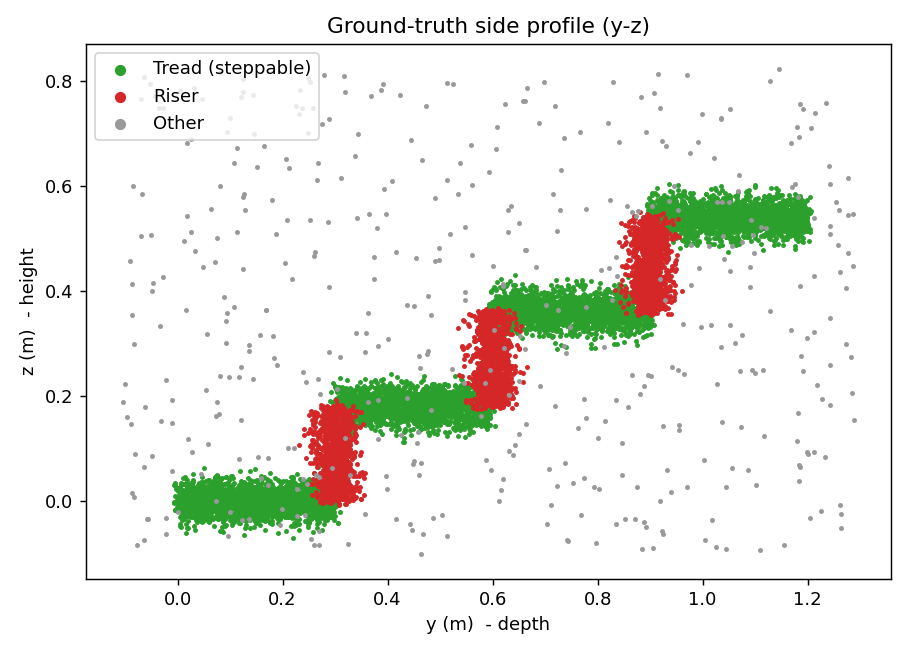
\includegraphics[width=0.95\columnwidth]{profile_ground_truth.png}
\caption{Side profile ($y$--$z$) of the ground-truth cloud: green = tread, red = riser, grey = other.}
\label{fig:profile}
\end{figure}

The steppable surface is the safety-critical class, so we score every
method on the tread label in a one-vs-rest setting: tread points are
positives, and all riser and ``other'' points are negatives.
Let $TP$, $FP$, $FN$, and $TN$ denote the per-point true positives, false
positives, false negatives, and true negatives. We report five standard
quantities, each computed for the tread class under this one-vs-rest
scheme. The tabulated accuracy $\mathrm{Acc}=(TP{+}TN)/(TP{+}TN{+}FP{+}FN)$
is the fraction of points placed correctly inside or outside the tread
class. In the text we also quote the overall \emph{three-class} accuracy,
the fraction of all points whose full tread/riser/other label is correct;
this differs from the one-vs-rest $\mathrm{Acc}$ of
Table~\ref{tab:metrics}. Precision
$\mathrm{P}=TP/(TP{+}FP)$ is the fraction of predicted tread points that
are genuinely treads, while recall $\mathrm{R}=TP/(TP{+}FN)$ is the
fraction of true tread points recovered. The F1 score is their harmonic
mean, $\mathrm{F1}=2\mathrm{P}\mathrm{R}/(\mathrm{P}{+}\mathrm{R})$, and the
intersection-over-union, or Jaccard index,
$\mathrm{IoU}=TP/(TP{+}FP{+}FN)$, expresses the spatial overlap between the
predicted and ground-truth tread regions. Precision and IoU matter most
for robotic foothold reasoning, because they directly measure how often a
non-steppable surface is taken for a steppable one.

Reproducibility was a design goal. The data generator and every stochastic
component of the pipeline (RANSAC sampling, neighbour selection, and the
noise draws) ran from a fixed pseudo-random seed, so the cloud and all
reported numbers regenerate deterministically. Method hyper-parameters
stayed constant across runs: RANSAC used an inlier threshold
$\tau=0.035$\,m, PCA normals were estimated from $k=50$ neighbours, and
DBSCAN used $\varepsilon=0.08$\,m within each orientation group.

\subsection{Results}

Table~\ref{tab:metrics} summarises the tread-class performance of the four
methods, and Fig.~\ref{fig:bars} places their F1 and IoU scores side by
side.

\begin{table}[t]
\caption{Tread-class segmentation metrics (one-vs-rest). Acc is one-vs-rest
tread accuracy, distinct from the three-class accuracy quoted in the text.
Best per column in bold.}
\label{tab:metrics}
\centering
\begin{tabular}{lccccc}
\toprule
Method & Acc & Prec & Rec & F1 & IoU \\
\midrule
RANSAC          & 0.681 & 0.714 & 0.904 & 0.798 & 0.664 \\
PCA-Normals     & 0.901 & \textbf{0.954} & 0.901 & 0.927 & 0.864 \\
DBSCAN-Slope    & \textbf{0.920} & 0.936 & 0.949 & \textbf{0.943} & \textbf{0.892} \\
Height-Histogram& 0.827 & 0.809 & \textbf{0.984} & 0.888 & 0.799 \\
\bottomrule
\end{tabular}
\end{table}

\begin{figure}[t]\centering
\begin{tikzpicture}
\begin{axis}[width=\columnwidth,height=4.6cm,ybar,bar width=6pt,ymin=0,ymax=1,
  symbolic x coords={RANSAC,PCANormals,DBSCANSlope,HeightHistogram},
  xtick=data,xticklabel style={rotate=20,anchor=east,font=\footnotesize},
  ylabel={score},legend pos=south east,enlarge x limits=0.15]
\addplot table[x=method,y=f1]{data/metrics.dat}; \addlegendentry{F1}
\addplot table[x=method,y=iou]{data/metrics.dat}; \addlegendentry{IoU}
\end{axis}
\end{tikzpicture}
\caption{Per-method tread-class F1 and IoU.}
\label{fig:bars}
\end{figure}

The orientation-aware \textbf{DBSCAN-Slope} method leads overall. It
attains the best F1 ($0.943$) and IoU ($0.892$) and the highest three-class
accuracy ($0.909$). The reason is its order of operations: by first
splitting the cloud into horizontal and vertical orientation groups and
clustering spatially only afterwards, it recovers each physical surface as
a single compact cluster and absorbs outliers into the noise label. The
result is a balanced precision ($0.936$) and recall ($0.949$).
Figure~\ref{fig:seg3d} sets the DBSCAN-Slope segmentation against the
ground truth; the individual treads separate cleanly, and riser
bleed-through is minimal.

\begin{figure}[t]\centering
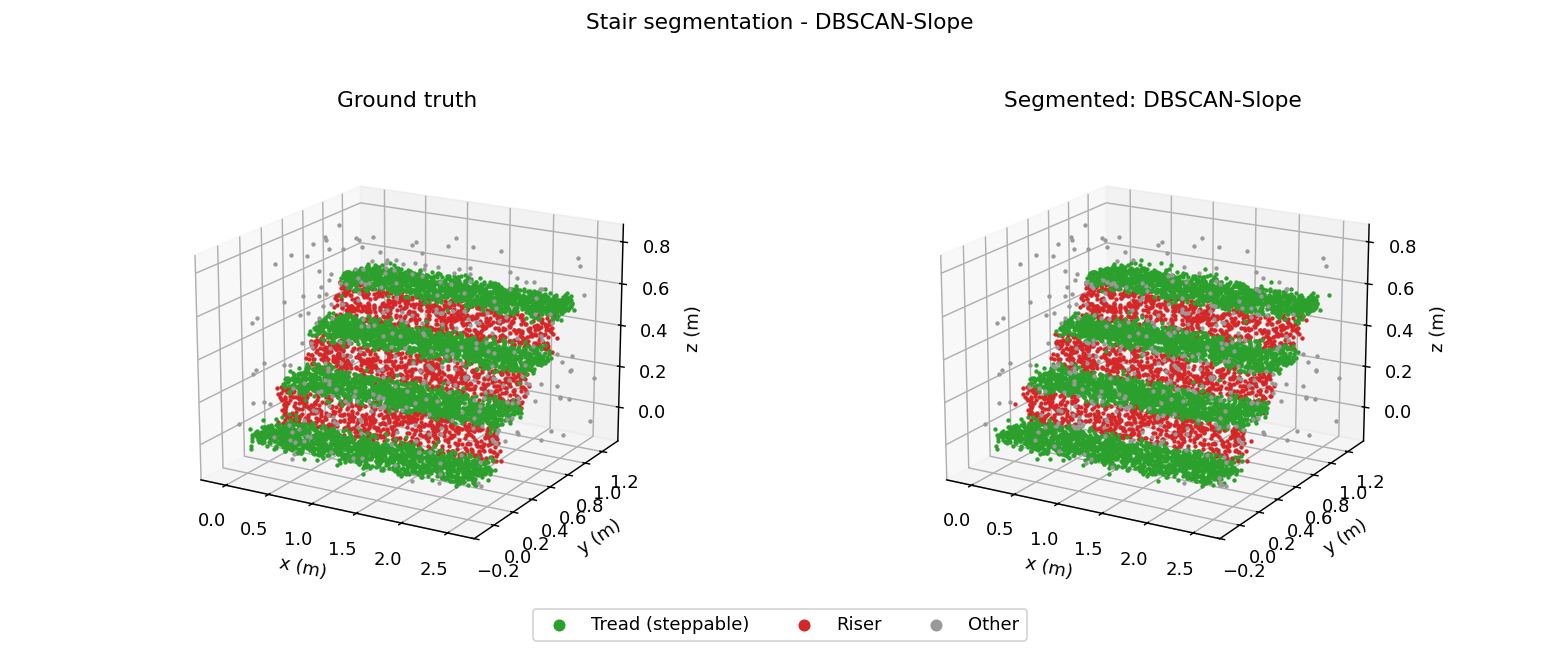
\includegraphics[width=\columnwidth]{seg_dbscan_slope.png}
\caption{3D segmentation by DBSCAN with slope analysis (right) vs.\ ground truth (left).}
\label{fig:seg3d}
\end{figure}

The \textbf{PCA-Normals} method follows close behind, with F1 $0.927$ and
IoU $0.864$. It classifies points directly from the local surface
orientation $|\nvec^\top\zhat|$, and this earns it the highest precision of
any method ($0.954$): a point is labelled tread only when its estimated
normal is nearly vertical, so very few risers slip through. Recall
($0.901$) sits marginally below DBSCAN's, because normals estimated near
tread--riser edges grow unreliable and a fraction of genuine tread points
fall outside the horizontal gate. The narrow gap between PCA-Normals and
DBSCAN-Slope confirms that local geometric orientation is an effective,
robust cue for separating the two principal surface types.

The \textbf{Height-Histogram} method acts as a high-recall,
lower-precision detector. It reaches the best recall of any method
($0.984$) but a markedly lower precision ($0.809$), giving F1 $0.888$ and
IoU $0.799$. Figure~\ref{fig:hist} shows the $z$-histogram, whose four
pronounced peaks correspond to the detected tread levels at
$z\approx\{0.00,0.18,0.36,0.54\}$\,m, close to the nominal step heights.
The method captures almost every tread point because treads concentrate
sharply at these levels. The trouble is that the horizontal bands it
assigns around each peak also enclose riser points whose vertical extent
happens to pass through a tread height, and that drags precision down.

\begin{figure}[t]\centering
\begin{tikzpicture}
\begin{axis}[width=\columnwidth,height=4.2cm,xlabel={$z$ (m)},ylabel={count},
  ymin=0,ymax=760,xmin=-0.1,xmax=0.65,enlarge x limits=false,tick label style={font=\footnotesize}]
\addplot[draw=blue!60!black,fill=blue!25] table[x=z,y=count]{data/hist.dat} \closedcycle;
\draw[green!55!black,dashed,thick] (axis cs:0.004,0) -- (axis cs:0.004,760);
\draw[green!55!black,dashed,thick] (axis cs:0.183,0) -- (axis cs:0.183,760);
\draw[green!55!black,dashed,thick] (axis cs:0.362,0) -- (axis cs:0.362,760);
\draw[green!55!black,dashed,thick] (axis cs:0.541,0) -- (axis cs:0.541,760);
\end{axis}
\end{tikzpicture}
\caption{Height histogram of $z$; dashed lines mark the four detected tread levels.}
\label{fig:hist}
\end{figure}

Plain \textbf{RANSAC} plane fitting is the weakest performer. It posts the
lowest precision ($0.714$), F1 ($0.798$), IoU ($0.664$), and three-class
accuracy ($0.667$), even with a high recall ($0.904$). One failure mode
dominates: the large horizontal planes RANSAC fits at each tread height
also swallow riser points that lie within the inlier band $\tau$ at those
heights. These mislabelled risers inflate the false-positive count and
collapse precision. The contrast with PCA-Normals is telling. A global
planar fit cannot tell a riser point that merely sits near a tread plane
from a true tread point, whereas a local normal can. This is why the
per-point orientation cues in PCA-Normals and DBSCAN-Slope beat the purely
planar formulation.

\subsection{Noise Sensitivity}

To probe robustness, we swept the height-noise standard deviation
$\sigma_z$ from $0.01$\,m to $0.07$\,m and re-evaluated PCA-Normals, whose
accuracy hinges most directly on the fidelity of local geometry. We vary
$\sigma_z$ rather than the riser depth jitter $\sigma_y$ because vertical
jitter is the axis that erodes the tread/riser orientation contrast,
whereas $\sigma_y$ mostly broadens riser planes without moving tread points
across step levels. Figure~\ref{fig:noise} plots the resulting tread-class
F1 and IoU.

\begin{figure}[t]\centering
\begin{tikzpicture}
\begin{axis}[width=\columnwidth,height=4.4cm,xlabel={$\sigma_z$ (m)},
  ylabel={tread-class score},ymin=0,ymax=1,legend pos=south west,
  grid=major,tick label style={font=\footnotesize}]
\addplot[blue,mark=*] table[x=sigma,y=f1]{data/noise.dat}; \addlegendentry{F1}
\addplot[red,mark=square*] table[x=sigma,y=iou]{data/noise.dat}; \addlegendentry{IoU}
\end{axis}
\end{tikzpicture}
\caption{Tread-class F1 and IoU versus height noise $\sigma_z$ (PCA-Normals).}
\label{fig:noise}
\end{figure}

Performance degrades monotonically, and the slope steepens as the noise
grows. At $\sigma_z=0.01$\,m the method is near-ideal (F1 $0.956$, IoU
$0.915$), and it holds up well through $\sigma_z=0.02$--$0.03$\,m. Past that
point the decline accelerates, reaching F1 $0.543$ and IoU $0.373$ at
$\sigma_z=0.07$\,m. The mechanism is geometric. The discriminative cue is
the near-vertical tread normal, but once $\sigma_z$ approaches half the step
height ($h/2=0.09$\,m), vertical jitter on tread points becomes comparable
to the vertical gap between adjacent steps. The local neighbourhoods used
for normal estimation then mix points from neighbouring treads and the
intervening riser, the estimated normals tilt away from vertical, the
horizontal orientation gate misfires, and tread and riser turn
geometrically indistinguishable. This marks a practical operating limit:
reliable tread segmentation needs the sensor's per-point height noise to
stay well below the step height it must resolve.

\subsection{Limitations and Threats to Validity}

Several limitations bound these conclusions. The benchmark is synthetic, a
single straight-flight, rectangular staircase with one fixed geometry
$(w,d,h,N)$ and an idealised, axis- and gravity-aligned layout. The
absolute scores should therefore be read as \emph{relative} method
rankings, not field-deployable accuracies. The sensor model is also
simplified: nominal Gaussian jitter plus uniform outliers, with no
occlusion, missing returns, incidence-angle effects, multi-path, or the
structured scan patterns of a real LiDAR. The height-histogram method, for
its part, assumes a regular, gravity-aligned staircase and would not
transfer to spiral, open-riser, or unaligned scans without modification.
Finally, every hyper-parameter ($\tau$, $k$, $\varepsilon$, the orientation
gates, and the histogram window) was tuned once on this cloud, and the
sensitivity study varies only $\sigma_z$ for a single method, so we make no
claim of cross-configuration parameter robustness. These constraints
motivate the real-sensor validation identified in
Section~\ref{sec:conclusion}.

\subsection{Safety Discussion for Stair-Following Robots}

For a stair-climbing or stair-following robot, the worth of these results
lies less in the average score than in the failure modes they expose. The
best method reaches IoU $\approx 0.89$, enough to support \emph{coarse}
foothold planning: the extracted tread regions overlap the true steppable
surfaces strongly enough for an elevation-map-based planner to place
candidate footholds on the correct steps, in line with practice in legged
and wheeled terrain perception
\cite{chavezgarcia2017learning,gomes2023survey}. Yet no method reaches unit
precision, and the dominant errors are exactly the dangerous ones: riser
points occasionally read as steppable. Inside a closed control loop such
false positives can lead a controller to commit a foothold to a vertical
face, the very failure mode that motivates dedicated stair perception
\cite{matsumura2022deep}.

We therefore recommend that a deployed system treat the raw per-point
labels as a hypothesis rather than a command. Three mitigations follow
directly from our findings. The first is \emph{ensemble voting} across
methods. Because the methods fail in complementary ways (RANSAC and the
histogram over-include risers, while PCA-Normals stays conservative),
voting can suppress method-specific false positives and combine the
histogram's high recall with the precision of the normal-based gate.
The second is a \emph{tread-edge erosion margin}. Mislabelling concentrates
at tread--riser boundaries, so shrinking each accepted tread region inward
before foothold selection trades a small amount of usable surface for a
sharp drop in the chance of stepping onto an edge or riser.
The third is \emph{temporal verification}. Given the strong noise
sensitivity established above, accumulating evidence across consecutive
scans before committing a foothold guards against transient mislabels
caused by momentary high-noise frames. Together these measures convert a
segmentation that is accurate on average into one whose residual errors
lean toward the safe side, which is the right design objective for robots
that physically traverse stairs.

\section{Conclusion}
\label{sec:conclusion}
We presented a parametric, fully labeled staircase point-cloud benchmark together with an apples-to-apples comparison of four classical geometric methods: RANSAC plane fitting, PCA normal analysis, DBSCAN with slope confirmation, and height-histogram banding. All four operate under a unified three-class formulation of treads, risers, and other points. On the steppable tread class, orientation-aware DBSCAN with per-cluster slope confirmation was the strongest method, reaching an F1 of $0.943$ and an IoU of $0.892$, with PCA-normals a close second. These findings rest on a single synthetic staircase under a controlled noise model, so they should be read as relative method rankings pending real-sensor validation. RANSAC was the weakest, primarily because horizontal planes fitted at tread heights absorb riser points and depress precision to $0.714$; the height-histogram, by contrast, attained the highest recall but conflated riser bands with treads. A noise-sensitivity sweep on the PCA-Normals method showed that its performance holds up at realistic jitter but degrades sharply once the height noise approaches half the step height, with tread F1 falling from $0.956$ at $\sigma_z=0.01$\,m to $0.543$ at $\sigma_z=0.07$\,m.

From a safety standpoint, an IoU near $0.89$ is adequate for coarse foothold planning. Yet no method reached unit precision, so residual mislabeling of risers as steppable remains a hazard for stair-following robots and assistive devices, which argues for conservative tread-edge margins and downstream verification. Future work will pursue ensemble fusion of the complementary geometric cues to recover precision, validation on real LiDAR staircases beyond the synthetic generator, and a controlled comparison against learned point-cloud segmenters \cite{qi2016pointnet,sarker2024comprehensive} under low-label regimes, where the reproducibility and interpretability of classical methods matter most.


\bibliographystyle{IEEEtran}
\bibliography{refs}

\end{document}
